%%%%%%%%%%%%%%%%%%%%%%%%%%%%%%%%%%%%%%%
% Wenneker Resume/CV
% LaTeX Template
% Version 1.1 (19/6/2016)
%
% This template has been downloaded from:
% http://www.LaTeXTemplates.com
%
% Original author:
% Frits Wenneker (http://www.howtotex.com) with extensive modifications by 
% Vel (vel@LaTeXTemplates.com)
%
% License:
% CC BY-NC-SA 3.0 (http://creativecommons.org/licenses/by-nc-sa/3.0/
%
%%%%%%%%%%%%%%%%%%%%%%%%%%%%%%%%%%%%%%

%----------------------------------------------------------------------------------------
%	PACKAGES AND OTHER DOCUMENT CONFIGURATIONS
%----------------------------------------------------------------------------------------

\documentclass[a4paper,12pt]{article} % Font and paper size, changed from memoir to article

%%%%%%%%%%%%%%%%%%%%%%%%%%%%%%%%%%%%%%%%%
% Wenneker Resume/CV
% Structure Specification File
% Version 1.1 (19/6/2016)
%
% This file has been downloaded from:
% http://www.LaTeXTemplates.com
%
% Original author:
% Frits Wenneker (http://www.howtotex.com) with extensive modifications by 
% Vel (vel@latextemplates.com)
%
% License:
% CC BY-NC-SA 3.0 (http://creativecommons.org/licenses/by-nc-sa/3.0/)
%
%%%%%%%%%%%%%%%%%%%%%%%%%%%%%%%%%%%%%%%%%

%----------------------------------------------------------------------------------------
%	PACKAGES AND OTHER DOCUMENT CONFIGURATIONS
%----------------------------------------------------------------------------------------

\usepackage{XCharter} % Use the Bitstream Charter font
\usepackage[utf8]{inputenc} % RequiRoyalBlue for inputting international characters
\usepackage[T1]{fontenc} % Output font encoding for international characters

\usepackage[top=1cm,left=.1cm,right=1cm,bottom=1cm]{geometry} % Modify margins

\usepackage{graphicx} % RequiRoyalBlue for figures

\usepackage{flowfram} % RequiRoyalBlue for the multi-column layout

\usepackage{url} % URLs

\usepackage[usenames,dvipsnames]{xcolor} % RequiRoyalBlue for custom colours

\usepackage{tikz} % RequiRoyalBlue for the horizontal rule

\usepackage{enumitem} % RequiRoyalBlue for modifying lists
\setlist{noitemsep,nolistsep} % Remove spacing within and around lists

\setlength{\columnsep}{\baselineskip} % Set the spacing between columns

% Define the left frame (sidebar)
\newflowframe{0.25\textwidth}{\textheight}{0pt}{0pt}[left]
\newlength{\LeftMainSep}
\setlength{\LeftMainSep}{0.25\textwidth}
\addtolength{\LeftMainSep}{1\columnsep}
 
% Small static frame for the vertical line
\newstaticframe{1.5pt}{\textheight}{\LeftMainSep}{0pt}
 
% Content of the static frame with the vertical line
\begin{staticcontents}{1}
\hfill
\tikz{\draw[loosely dotted,color=RoyalBlue,line width=1.5pt,yshift=0](0,0) -- (0,\textheight);}
\hfill\mbox{}
\end{staticcontents}
 
% Define the right frame (main body)
\addtolength{\LeftMainSep}{1.5pt}
\addtolength{\LeftMainSep}{1\columnsep}
\newflowframe{0.7\textwidth}{\textheight}{\LeftMainSep}{0pt}[main01]

\pagestyle{empty} % Disable all page numbering

\setlength{\parindent}{0pt} % Stop paragraph indentation

%----------------------------------------------------------------------------------------
%	NEW COMMANDS
%----------------------------------------------------------------------------------------

\newcommand{\userinformation}[1]{\renewcommand{\userinformation}{#1}} % Define a new command for the CV user's information that goes into the left column

\newcommand{\cvheading}[1]{{\Huge\bfseries\color{RoyalBlue} #1} \par\vspace{.6\baselineskip}} % New command for the CV heading
\newcommand{\cvsubheading}[1]{{\Large\bfseries #1} \bigbreak} % New command for the CV subheading

\newcommand{\Sep}{\vspace{1em}} % New command for the spacing between headings
\newcommand{\SmallSep}{\vspace{0.5em}} % New command for the spacing within headings

\newcommand{\aboutme}[2]{ % New command for the about me section
\textbf{\color{RoyalBlue} #1}~~#2\par\Sep
}
	
\newcommand{\CVSection}[1]{ % New command for the headings within sections
{\Large\textbf{#1}}\par
\SmallSep % Used for spacing
}

\newcommand{\CVItem}[2]{ % New command for the item descriptions
\textbf{\color{RoyalBlue} #1}\par
#2
\SmallSep % Used for spacing
}

\newcommand{\bluebullet}{\textcolor{RoyalBlue}{$\circ$}~~} % New command for the blue bullets
 % Include the file specifying document layout and packages
\usepackage{graphicx}
\usepackage{tabu}
%----------------------------------------------------------------------------------------
%	NAME AND CONTACT INFORMATION 
%----------------------------------------------------------------------------------------

\userinformation{ % Set the content that goes into the sidebar of each page
\begin{flushright}
% Comment out this figure block if you don't want a photo
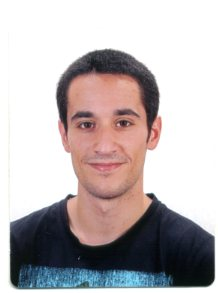
\includegraphics[width=0.6\columnwidth]{fede_fototessera.jpg}\\[\baselineskip] % Your photo
\small % Smaller font size
Federico Massa \\ % Your name
\url{fedemassa91@gmail.com}  \\
%\url{gmail.com} \\ % Your email address
%\url{www.johnsmith.com} \\ % Your URL
(+39) 347-7034248 \\ % Your phone number
\Sep % Some whitespace
\textbf{Address} \\
Via G. B. Pellizzi, 6 \\ % Address 1
56127 Pisa (PI) \\ % Address 2
Italy \\ % Address 3
\vfill % Whitespace under this block to push it up under the photo
\end{flushright}
}

%----------------------------------------------------------------------------------------

\begin{document}

\userinformation % Print your information in the left column

\framebreak % End of the first column

%----------------------------------------------------------------------------------------
%	HEADING
%----------------------------------------------------------------------------------------

\cvheading{Federico Massa} % Large heading - your name

\cvsubheading{Physicist} % Subheading - your occupation/specialization

%----------------------------------------------------------------------------------------
%	ABOUT ME
%----------------------------------------------------------------------------------------

%----------------------------------------------------------------------------------------
%	EDUCATION
%----------------------------------------------------------------------------------------

\CVSection{Education}

%------------------------------------------------

\CVItem{2013 - 2016, Universit\`a di Pisa}{MSc in Physics of Fundamental Interactions - 110/110 cum laude.\\
- Thesis title: ``Tracking performances of the ATLAS detector for the HL-LHC and impact on 
the H $\rightarrow 4\mu$ channel''.}

%------------------------------------------------


\CVItem{2010 - 2013, Universit\`a degli Studi di Cagliari}{BSc in Physics - 110/110 cum laude.\\
- Thesis title: ``Impact of physics beyond the Standard Model on the diffusion of neutrinos on polarized electrons''.}

%------------------------------------------------

\CVItem{2005 - 2010, Liceo Scientifico Pitagora - Selargius (CA)}{High School Diploma (Diploma di Maturit\`a Scientifica) - 100/100 cum laude.}

\CVSection{Experiences}

\CVItem{Jun 2016: Alghero}{Attendance to the XIII Seminar on Nuclear, Subnuclear and Applied Physics}

\CVItem{Aug 2014: Göttingen}{Attendance to the HASCO Summer School on Hadron Colliders}
%\Sep % Extra whitespace after the end of a major section

%----------------------------------------------------------------------------------------
%	EXPERIENCE
%----------------------------------------------------------------------------------------

%\CVSection{Experience}

%------------------------------------------------

%------------------------------------------------

%------------------------------------------------

\Sep % Extra whitespace after the end of a major section

%----------------------------------------------------------------------------------------
%	COMMUNICATION SKILLS
%----------------------------------------------------------------------------------------
\CVSection{Languages}
\begin{table}[h!]
\centering
\resizebox{.71\textwidth}{!}{\tabulinesep=1.2mm{\begin{tabu}{| l | c | c | c | c | c |}
\cline{2-6}
\multicolumn{1}{c}{ } & \multicolumn{2}{|c|}{\textbf{Understanding}} & \multicolumn{2}{c|}{\textbf{Speaking}} & \textbf{Writing} \\ \cline{2-6}
\multicolumn{1}{c}{ } & \multicolumn{1}{|c|}{Listening} & Reading & Spoken interaction & Spoken production & \\ \hline
English & C1 & C1 & C1 & C1 & C1 \\ \hline
Spanish & B2 & B2 & B2 & B2 & B2 \\ \hline
\end{tabu}}}
\end{table}

The corresponding certificates can be found in the attachments.

\Sep 

\CVSection{Communication Skills}

%------------------------------------------------

\CVItem{2015-2016, \textit{Oral Presentations}}{During my Master's Degree thesis,
 I presented my work a large number of times to different research groups of
 the ATLAS experiment: 
 \begin{itemize}
 \item ATLAS Pisa;
 \item ITk Simulation \& Performance;
 \item Upgrade Tracking;
 \item Physics Upgrade;
 \item ITk Layout Taskforce.
 \end{itemize}
 }

%------------------------------------------------
\Sep
I really enjoy, and I have a many years' experience in teaching Physics and Mathematics to students from Middle School to BSc.\\

%------------------------------------------------

%\Sep % Extra whitespace after the end of a major section

%----------------------------------------------------------------------------------------
%	SKILLS
%----------------------------------------------------------------------------------------

\clearpage
\userinformation
\framebreak

\CVSection{Specific Skills}
\begin{itemize}
\item Mathematical analysis;
\item Classical and Quantum Mechanics;
\item Electromagnetism;
\item Statistical Data Analysis;
\item Experimental techniques;
\item Fundamentals of Analog and Digital Electronics;
\item Monte Carlo simulations;
\item Image processing and Computer Vision.
\end{itemize}

\Sep 

\CVSection{Software Skills}

%------------------------------------------------

\CVItem{Programming}
{\begin{tabular}{p{0.2\textwidth} p{0.2\textwidth} p{0.2\textwidth}}
\bluebullet C++ &  \bluebullet Java & \bluebullet Unix shell\\
\bluebullet Python &  \bluebullet Mathematica & \bluebullet Matlab\\
\bluebullet Fortran 90 & \bluebullet Visual Basic & C\\
\end{tabular}}

%------------------------------------------------

\CVItem{Operative systems}
{\begin{tabular}{p{0.2\textwidth} p{0.2\textwidth} p{0.2\textwidth}}
 \bluebullet Windows &  \bluebullet Linux & \bluebullet Android\\
\end{tabular}}

%-----------------------------------------------

\CVItem{Computer software}
{\begin{tabular}{p{0.2\textwidth} p{0.2\textwidth} p{0.2\textwidth}}
 \bluebullet Internet browsers & \bluebullet Microsoft Office & \bluebullet LaTeX \\
 \bluebullet ROOT Framework & \bluebullet Geant4 & \bluebullet Gnuplot \\
 \bluebullet Qt Creator & \bluebullet Eclipse & \bluebullet Android Studio \\
\end{tabular}}

Among the programming languages, I know C++ and Java particularly well.

%------------------------------------------------

\Sep % Extra whitespace after the end of a major section

%----------------------------------------------------------------------------------------
%	NEW PAGE DELIMITER
%	Place this block wherever you would like the content of your CV to go onto the next page
%----------------------------------------------------------------------------------------

%----------------------------------------------------------------------------------------
%	AWARDS
%----------------------------------------------------------------------------------------

%\CVSection{Awards}

%------------------------------------------------

%\CVItem{2010, \textit{Postgraduate Scholarship}, Cornell University}{Awarded to the top student in their final year of a Bachelors degree.}

%------------------------------------------------

%\Sep % Extra whitespace after the end of a major section

%----------------------------------------------------------------------------------------
%	INTERESTS
%----------------------------------------------------------------------------------------

\CVSection{Interests}

%------------------------------------------------

\CVItem{Professional}{Software and app development, Artificial Intelligence, 
Automation, Software simulation of physical systems.}

%------------------------------------------------

\CVItem{Personal}{Arduino programming, Android apps development, Jazz music, piano, 
sports, video-games.}

%------------------------------------------------

\Sep % Extra whitespace after the end of a major section

%----------------------------------------------------------------------------------------
\CVSection{Attachments}

\textit{BSc academic transcript}\\
\textit{MSc academic transcript}\\
\textit{Alghero seminar examination certificate}\\
\textit{English language certificate}\\
\textit{Spanish language certificate}\\


\end{document}
